\section{Organización de los resultados}
Como se explicó en los capítulos anteriores, las propuestas planteadas en este trabajo son de dos tipos: modificar el paisaje de búsqueda del problema y cambiar la metaheurística con la que se explora este paisaje.
En el caso de la metaheurística la única modificación es usar la búsqueda local iterada (ILS). Para el caso del paisaje de búsqueda se presentan varias modificaciones a cada una de sus componentes: representación de soluciones, estructura de vecindad y función de fitness.

En primer lugar se presenta el cambio en metaheurística utilizando la representación basada en permutaciones y la vecindad N7, seguido del cambio en la función de fitness. Posteriormente se considera la extensión planteada a la vecindad N7 y por último la representación basada en llaves aleatorias junto con la nueva vecindad propuesta. Se asignan acrónimos a cada variante para facilitar la comparación. El orden de presentación es el siguiente:
\begin{enumerate}
    \item \textbf{PN7Cmax} Representación basada en permutaciones, vecindad N7 y makespan como función de fitness.
    \item \textbf{PN7*} Representación basada en permutaciones, vecindad N7 y diversas funciones de fitness.
    \item \textbf{PN7extTup} Representación basada en permutaciones, vecindad N7 extendida y tupla ordenada de tiempos de finalización como función de fitness.
    \item \textbf{RpKeTup} Representación basada en llaves aleatorias, vecindad propuesta y tupla ordenada de tiempos de finalización función de fitness.
\end{enumerate}

Cada una de las variaciones propuestas se ejecutó durante 5 minutos por 50 veces para cada instancia del conjunto \textbf{DMU01-80} con el fin de obtener un conjunto de resultados para comparar.

Puesto que el objetivo de las modificaciones planteadas en este trabajo es presentar una alternativa simple a los métodos del estado del arte pero sin perder calidad en las soluciones, se presenta la mediana del error relativo respecto al mejor resultado reportado en la literatura. El mejor resultado reportado en la literatura para cada instancia se muestra en el apéndice \ref{tab:sota}.
El error relativo se calcula entonces de la siguiente manera: \[\text{error relativo}= \frac{\text{mejor makespan en la literatura}-\text{makespan de la solución encontrada}}{\text{\text{mejor makespan en la literatura}}}\]

\section{Resultados para PN7Cmax}
Estos resultados sirven como una base para determinar si las modificaciones posteriores resultan en mejoras apreciables puesto que el único cambio con los métodos más exitosos actualmente.

Se muestran los resultados de manera gráfica para facilitar su visualización. Los resultados detallados se encuentran en el apéndice \ref{app:resn7ils}. 

En la figura \ref{fig:PN7Cmax} podemos observar que la mediana del error relativo para la segunda mitad de las instancias es considerablemente mayor que para la primera mitad, en la cual en varios casos incluso se llegó a igualar el mejor resultado conocido.  
\begin{figure}[hbtp]
    \begin{subfigure}{\textwidth}
        \centering
        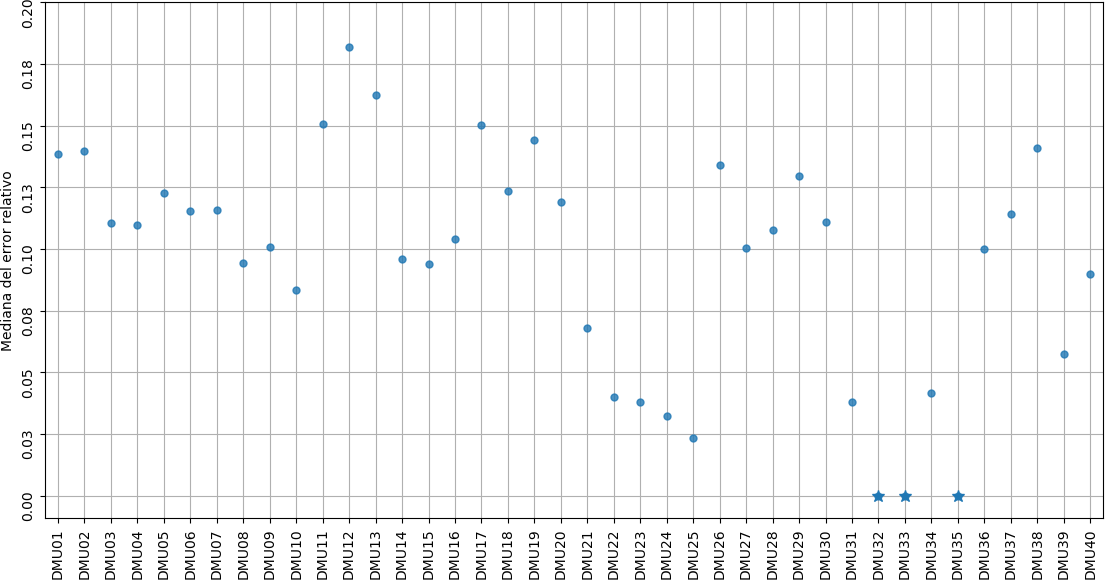
\includegraphics[scale=.65]{Imagenes/resn7ils1.png}
        \caption{Resultados para las instancias \textbf{DMU01-40}}
    \end{subfigure}
\end{figure}
\begin{figure}[H]\ContinuedFloat
    \begin{subfigure}{\textwidth}
        \centering
        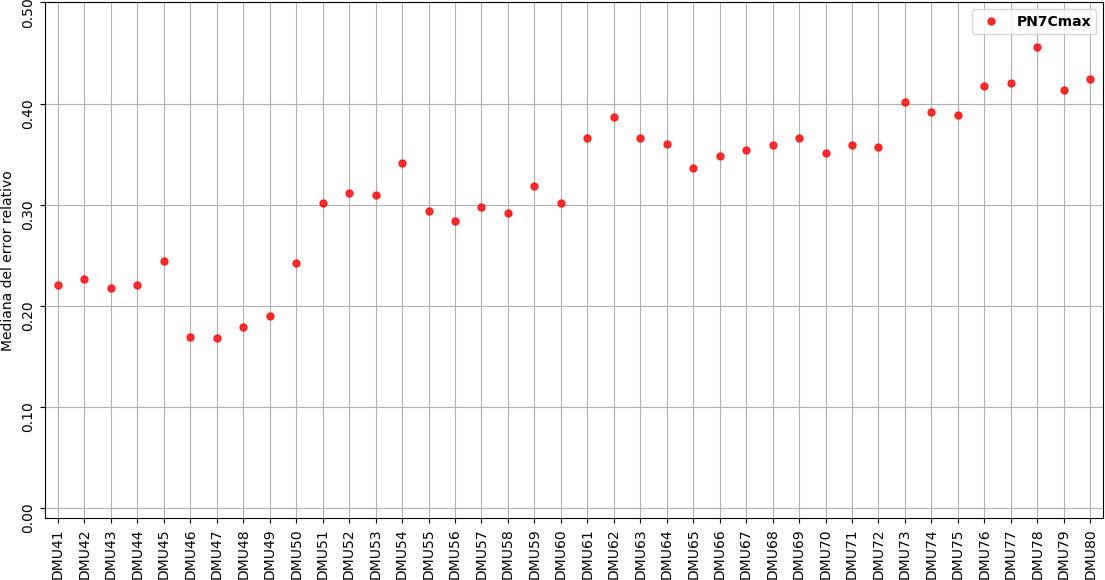
\includegraphics[scale=.65]{Imagenes/resn7ils2.png}
        \caption{Resultados para las instancias \textbf{DMU41-80}}
    \end{subfigure}
    \caption{Resultados para \textbf{PN7Cmax}. Se marcan los casos en los que se llegó a la mejor solución conocida.}
    \label{fig:PN7Cmax}
\end{figure}

Podemos observar que incluso usando una metaheurística simple por un corto tiempo podemos obtener resultados de calidad. En la siguiente sección podremos observar que la función de fitness puede ayudarnos a tener incluso mejores resultados.

\section{Resultados para distintas funciones de fitness}
  La función de fitness se obtiene al construir la dupla formada por el makespan y alguna característica en ese orden. Para determinar cuál es la que obtiene mejores resultados, las modificaciones se comparan a pares en cada instancia. Si se encuentra que la diferencia entre dos modificaciones es estadísticamente significativa, se le suma un punto a la ganadora y se le resta uno a la perdedora. De este modo cada variante de la función de fitness obtiene un puntaje que permite compararla con las demás.
Para determinar si los conjuntos de resultados muestran diferencias estadísticamente significativas se utiliza la prueba de Wilcoxon con un nivel de significancia de $0.01$. 

Los acrónimos asignados a cada una de las variantes que resultan de tomar las características propuestas se muestran en la tabla \ref{tab:caracter}.
\begin{table}[hbtp]
    \centering
\begin{tabular}{@{}cc@{}}
Característica                    & Acrónimo       \\ \hline \hline
$\mathbf{C_{max}}$ (makespan)     & \textbf{PN7Cmax}   \\\midrule
$\mathbf{\sum C_i^2}$             & \textbf{PN7C2}    \\\midrule
$\mathbf{\sum J_i}$               & \textbf{PN7Flow}  \\\midrule
$\mathbf{\sum I(C_i=C_{max})}$    & \textbf{PN7Icmax} \\\midrule
\textbf{Número de rutas críticas} & \textbf{PN7Rc}    \\\midrule
$\mathbf{Var(C_i)}$               & \textbf{PN7VarC}  \\\midrule
$\mathbf{(\{C_i\})}$              & \textbf{PN7Tup}    \\\midrule
\end{tabular}
    \caption{Acrónimos asignados a cada característica}
    \label{tab:caracter}
\end{table}

Los resultados para las propuestas mostradas en \ref{prop:fitness} pueden verse de manera condensada en la figura \ref{fig:fcomp}. La casilla $(i,j)$ muestra el número de veces que la variante $i$ fue mejor menos el número veces que fue peor que la variante $j$.\\
Se muestra también una tupla construida con las características que obtuvieron mejores resultados presentada como \textbf{PN7C2/Flow/VarC}. En la tabla \ref{tab:fcomp} se presentan ordenadas las variantes por el puntaje obtenido. Podemos observar que las primeras tres entradas están relativamente cerca aunque se ven diferencias claras entre ellas.\\

Podemos observar en la figura \ref{fig:fcomp} y en la tabla \ref{tab:fcomp} que el makespan fue la peor función de fitness. Para la tupla construida con las mejores características se observan pocas mejoras por lo que podemos concluir que agregar más características no lleva necesariamente a mejores resultados. Los mejores resultados se obtienen al construir la tupla de tiempos ordenados de finalización de las máquinas por lo que de ahora en adelante la función de fitness queda fija de esta manera y en los resultados subsecuentes solo se considera este caso. Los resultados detallados para esta función de fitness se muestran en el apéndice \ref{app:resn7tuple}.
Con estos resultados podemos concluir que es ventajoso enfocarse en mejorar las máquinas que tardan más tiempo siendo las tres mejores variantes las que toman más en cuenta estas máquinas.

\begin{figure}[hbtp]
    \centering
    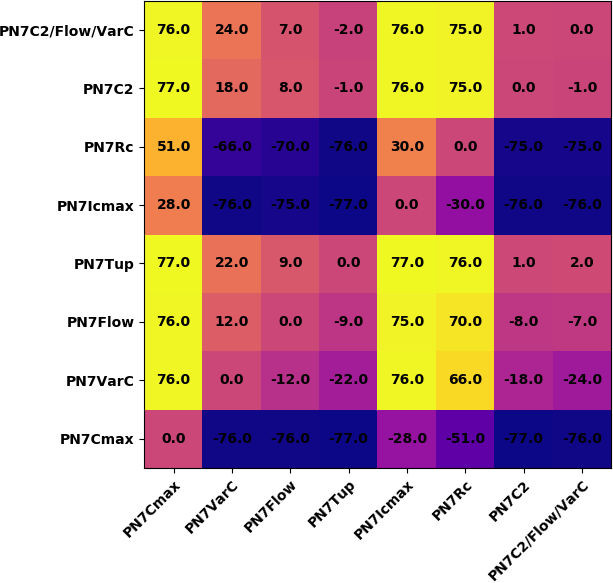
\includegraphics[scale=.8]{Imagenes/fitnesscomp.png}
    \captionof{figure}{Condensado de los resultados para las modificaciones a la función de fitness. }
    \label{fig:fcomp}
\end{figure}
\begin{table}[hbtp]
    \centering
\begin{tabular}{@{}cc@{}}
Variante & Puntaje \\ \midrule
\toprule
    \textbf{PN7Tup} & 264.0 \\ \midrule
    \textbf{PN7C2/flow/VarC} & 257.0 \\ \midrule
    \textbf{PN7C2} & 252.0 \\ \midrule
    \textbf{PN7Flow} & 209.0 \\ \midrule
    \textbf{PN7VarC} & 142.0 \\ \midrule
    \textbf{PN7Rc} & -281.0 \\ \midrule
    \textbf{PN7Icmax} & -382.0 \\ \midrule
    \textbf{PN7Cmax} & -461.0 \\ \midrule
\end{tabular}
    \caption{Puntaje para cada una de las variantes de función de fitness propuesta}
    \label{tab:fcomp}
\end{table}

Para mostrar de manera más concisa el efecto de la función de fitness en la calidad de las soluciones encontradas, en la figura \ref{fig:PN7CmaxvsPN7Tup} se muestra una comparación de los resultados hallados para la mejor función de fitness \textbf{PN7Tup} contra el caso base \textbf{PN7Cmax} que fue el que obtuvo peores resultados.
\begin{figure}[hbtp]
    \begin{subfigure}{\textwidth}
        \centering
        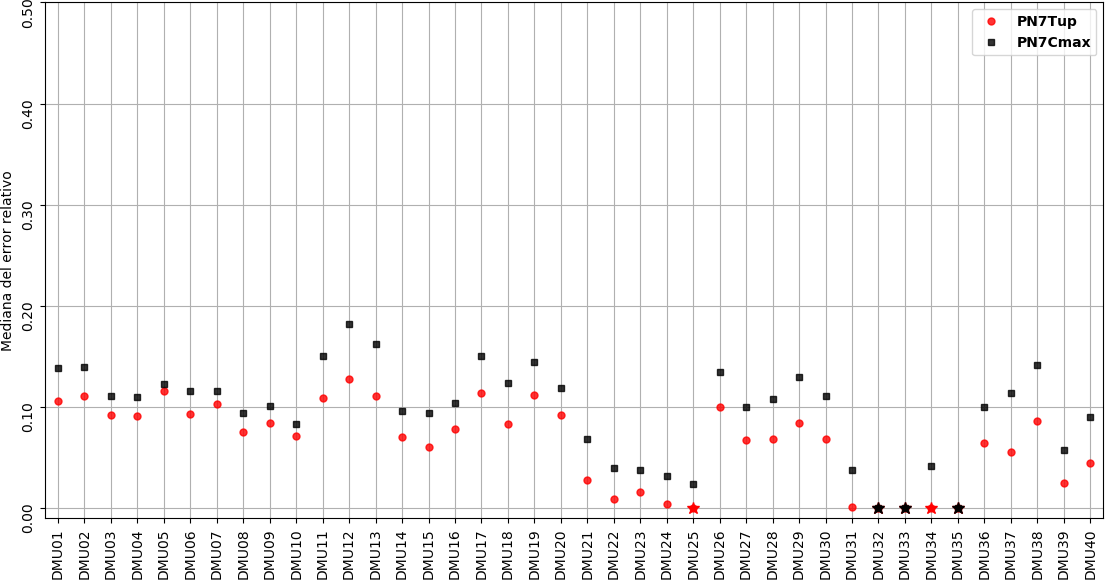
\includegraphics[scale=.65]{Imagenes/PN7CmaxvsPN7Tup_1.png}
        \caption{Resultados para las instancias \textbf{DMU01-40}}
    \end{subfigure}
\end{figure}
\begin{figure}[H]\ContinuedFloat
    \begin{subfigure}{\textwidth}
        \centering
        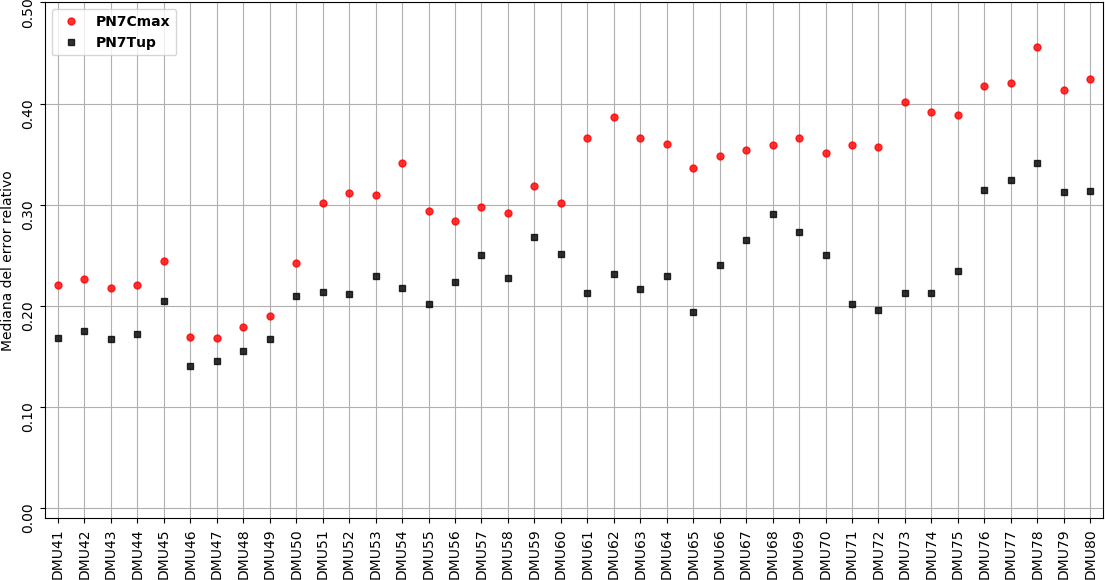
\includegraphics[scale=.65]{Imagenes/PN7CmaxvsPN7Tup_2.png}
        \caption{Resultados para las instancias \textbf{DMU41-80}}
    \end{subfigure}
    \caption{Comparación entre la peor y la mejor función de fitness. Se marcan los casos en los que se llegó a la mejor solución conocida.}
    \label{fig:PN7CmaxvsPN7Tup}
\end{figure}


\section{Resultados para PN7extTup}
Los resultados para la extensión a la vecindad N7 que considera movimientos que buscan aprovechar espacios de inactividad de las máquinas se comparan con los mejores mostrados en la sección pasada \textbf{PN7Tup}. Se sigue el mismo procedimiento que en la sección anterior para hacer esta comparación.
En la figure \ref{fig:n8vsn7} podemos observar que \textbf{PN7extTup} sí consigue mejorar los resultados obtenidos hasta el momento en varios casos. Esto nos indica que los movimientos considerados pueden o no llevar a mejores soluciones.

\begin{figure}[hbtp]
    \centering
    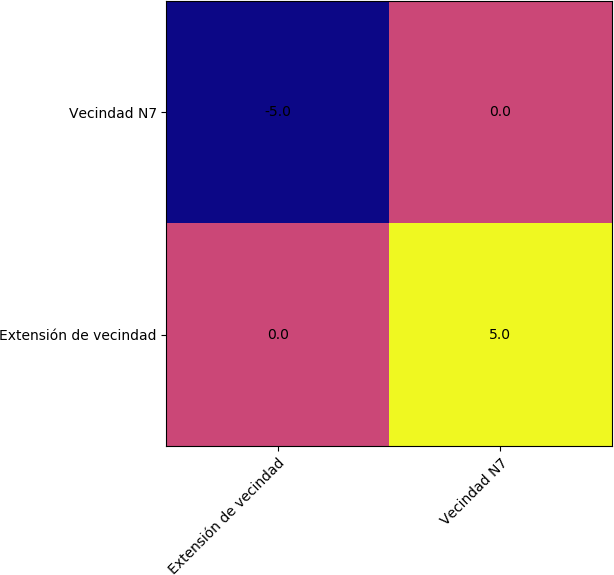
\includegraphics[scale=.7]{Imagenes/n8vsn7.png}
    \caption{Resultados de la comparación}
    \label{fig:n8vsn7}
\end{figure}

Aunque el puntaje obtenido por esta modificación fue positivo, en la figura \ref{fig:errn8vsn7} podemos observar que la mejora no es consistente ya que en algunos casos resulta peor que \textbf{PN7Tup} y en casi todas las instancias no presenta una disminución sustancial del error relativo por lo que se puede concluir que la extensión de la vecindad planteada no consigue beneficios importantes. Los resultados detallados para la \textbf{PN7extTup} se encuentran en el apéndice \ref{app:resn8tuple}.

\begin{figure}[hbtp]
    \begin{subfigure}{\textwidth}
        \centering
        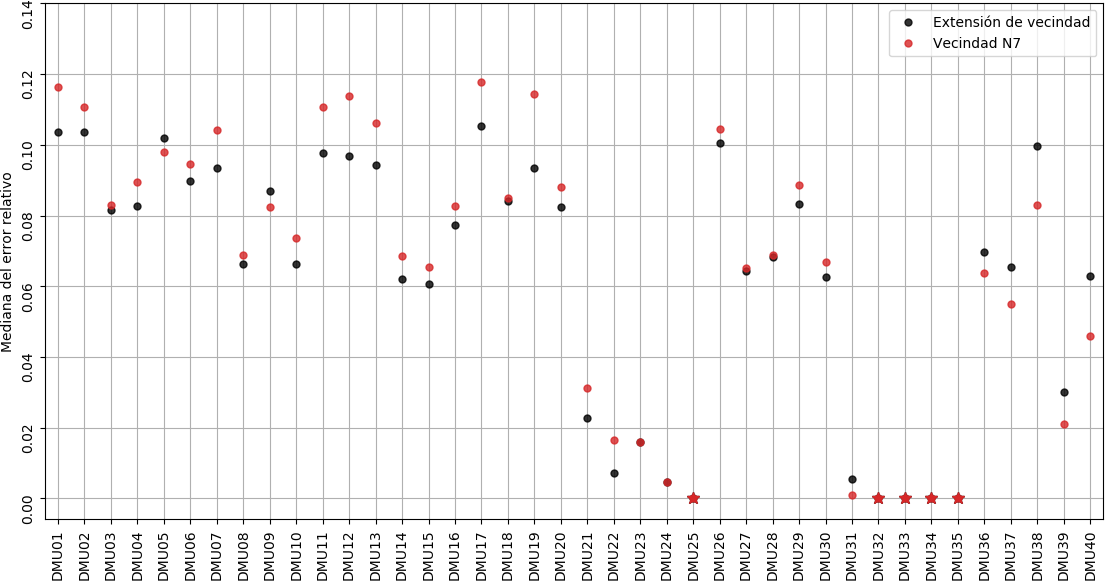
\includegraphics[scale=.6]{Imagenes/n8vsn7err1.png}
        \caption{Resultados para las instancias \textbf{DMU01-40}}
    \end{subfigure}
\end{figure}
\begin{figure}[H]\ContinuedFloat
    \begin{subfigure}{\textwidth}
        \centering
        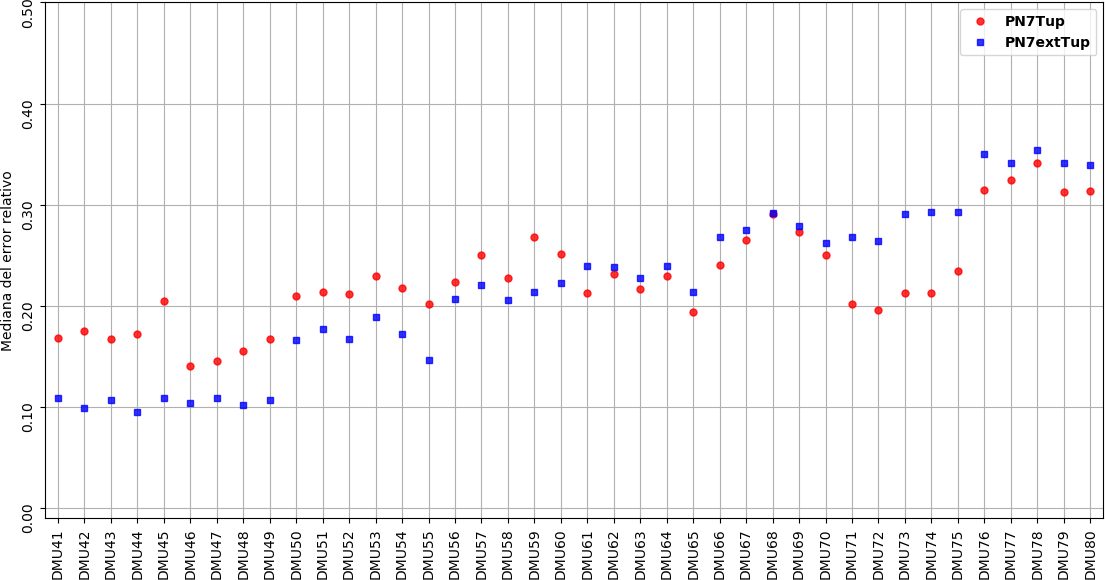
\includegraphics[scale=.6]{Imagenes/n8vsn7err2.png}
        \caption{Resultados para las instancias \textbf{DMU41-80}}
    \end{subfigure}
    \caption{Resultados para los métodos \textbf{PN7extTup} y \textbf{PN7Tup}. Se marcan los casos en los que se llegó a la mejor solución conocida.}
    \label{fig:errn8vsn7}
\end{figure}

\section{Cambio de representación y vecindad}
El cambio de representación y vecindad \textbf{RpKeTup} se compara con las dos propuestas previas: \textbf{PN7extTup} y \textbf{PN7Tup}. Se sigue el mismo procedimiento mencionado anteriormente para comparar y determinar si existe una diferencia significativa entre los resultados obtenidos. En la figura \ref{fig:n7vsn8vspr} y en la tabla \ref{tab:n7n8pr} podemos apreciar que \textbf{RpKeTup} presenta una ventaja aunque no muy grande. Los resultados detallados para \textbf{RpKeTup} se encuentran en el apéndice \ref{app:resprtuple}. 

\begin{figure}[hbtp]
    \centering
    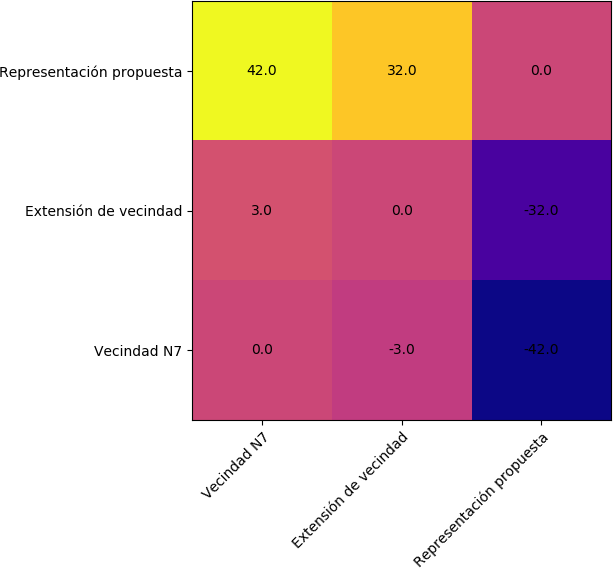
\includegraphics[scale=.7]{Imagenes/prn7n8comp.png}
    \caption{Resultados de la comparación entre los tres métodos.}
    \label{fig:n7vsn8vspr}
\end{figure}

\begin{table}[hbtp]
    \centering
\begin{tabular}{@{}cc@{}}
Variante & Puntaje \\ \midrule
\toprule
    \textbf{RpKeTup} & 37.0 \\ \midrule
    \textbf{PN7extTup} & 30.0 \\ \midrule
    \textbf{PN7Tup} & -67.0 \\ \midrule
\end{tabular}
    \caption{Puntaje total para cada método.}
    \label{tab:n7n8pr}
\end{table}

En la figura \ref{fig:n7vsn8vsprerr} podemos observar que la ventaja que tiene \textbf{RpKeTup} está concentrada en la segunda mitad de las instancias. Como se mencionó anteriormente, en las instancias \textbf{DMU41-80} todos los trabajos tienen operaciones iniciales en un mismo subconjunto de máquinas, la nueva representación toma en cuenta soluciones activas con lo que consigue evitar parcialmente el cuello de botella que resulta en soluciones de muy mala calidad.
\begin{figure}[hbtp]
    \begin{subfigure}{\textwidth}
        \centering
        %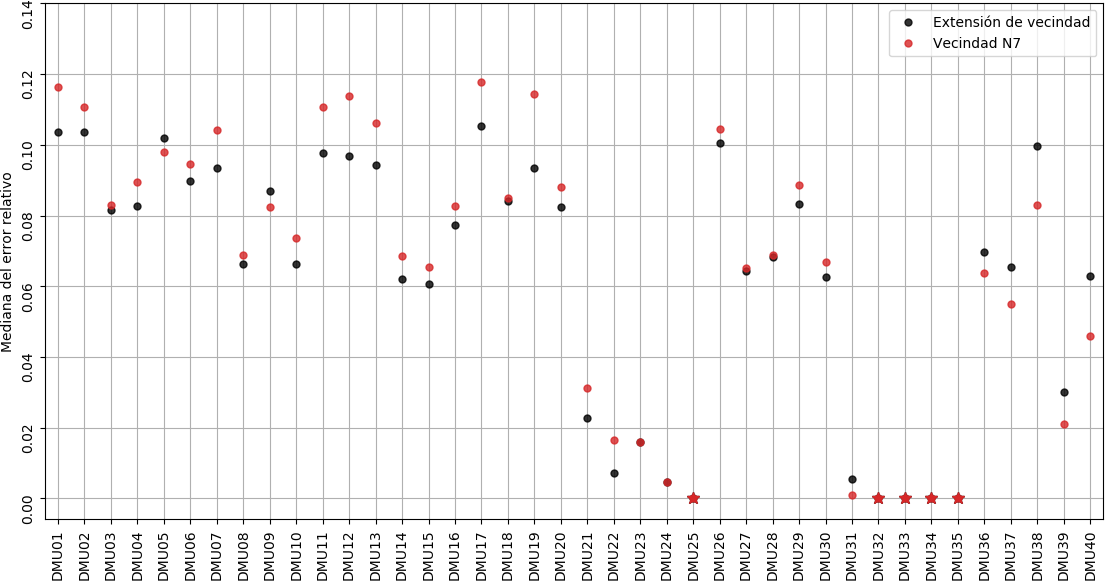
\includegraphics[height=.78\textwidth,width=.95\textheight,angle=270]{Imagenes/n8vsn7err1.png}
        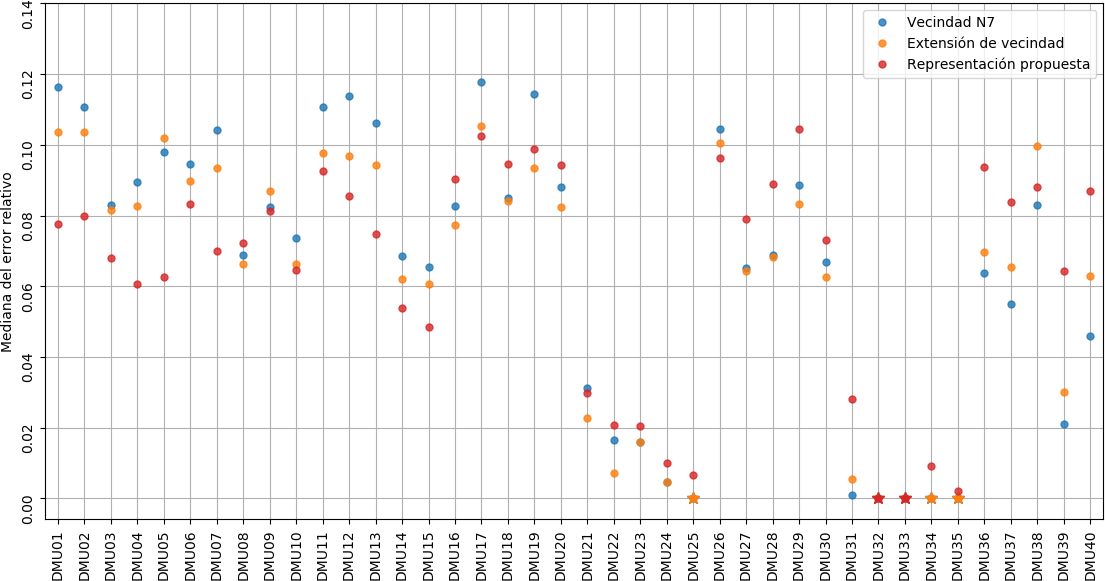
\includegraphics[scale=.6]{Imagenes/prvsn7vsn8err1.png}
        \caption{Resultados para las instancias \textbf{DMU01-40}}
    \end{subfigure}
\end{figure}
\begin{figure}[H]\ContinuedFloat
    \begin{subfigure}{\textwidth}
        \centering
        %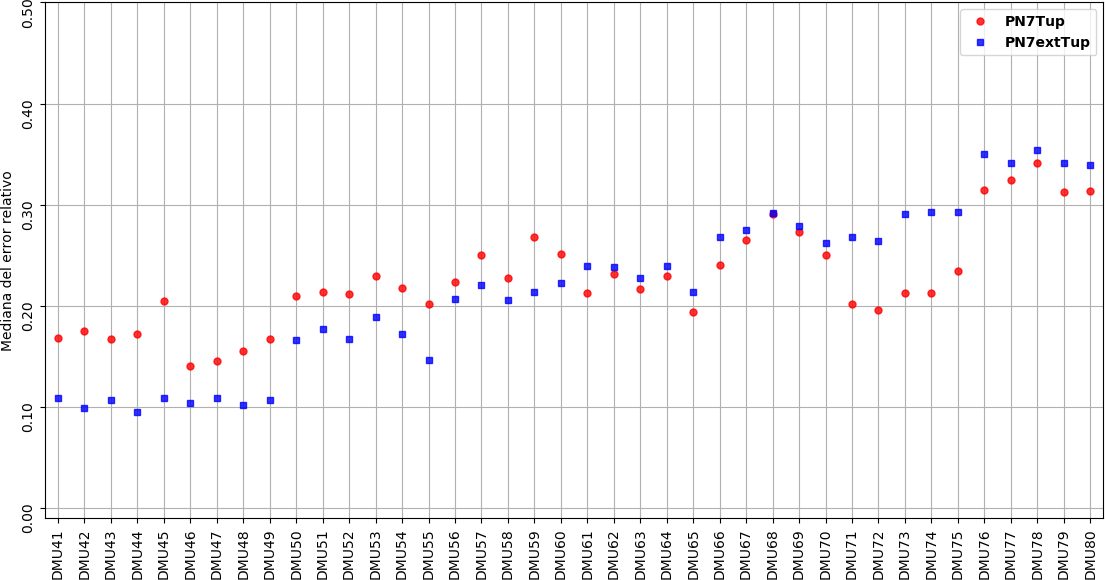
\includegraphics[height=.78\textwidth,width=.95\textheight,angle=270]{Imagenes/n8vsn7err2.png}
        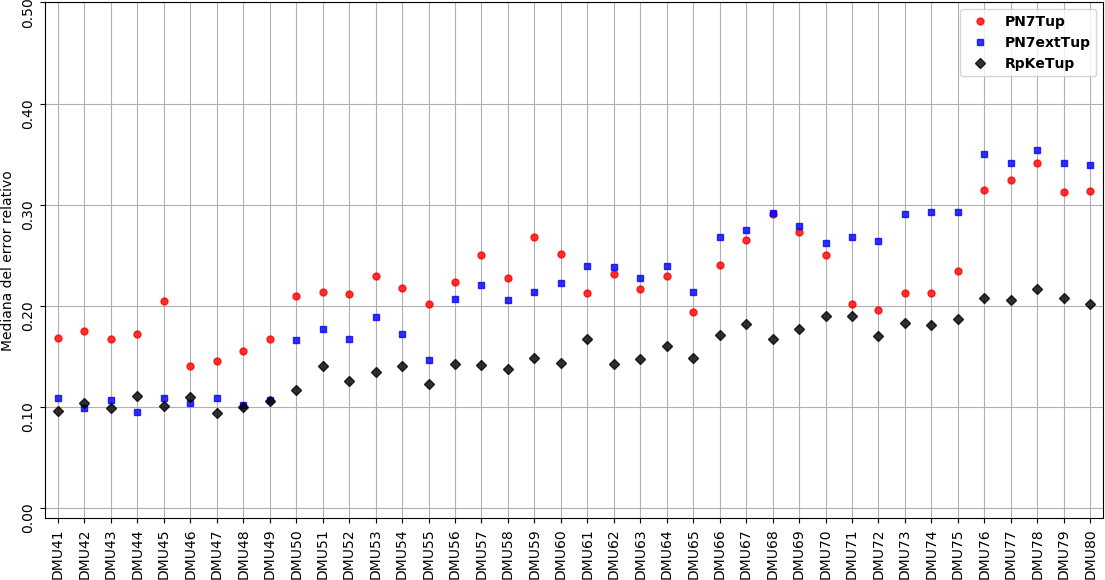
\includegraphics[scale=.6]{Imagenes/prvsn7vsn8err2.png}
        \caption{Resultados para las instancias \textbf{DMU41-80}}
    \end{subfigure}
    \caption{Resultados para \textbf{PN7Tup}, \textbf{PN7extTup} y \textbf{RpKeTup}. Se marcan los casos en los que se llegó a la mejor solución conocida.}
    \label{fig:n7vsn8vsprerr}
\end{figure}

Para resaltar las diferencias entre \textbf{RpKeTup} y \textbf{PN7Tup} se tomó la instancia en la que se obtuvieron los resultados más dispares (\textbf{DMU78}) y se para cada óptimo local visitado se registró su makespan así como el tamaño de su vecindad como se muestra en la figura \ref{fig:mattgraph}. Este procedimiento nos permite hacernos una idea de cómo se conectan las soluciones en función de su makespan. Lo más deseable es que los óptimos locales de alta calidad tengan vecindades grandes y los de mala calidad tengan vecindades pequeñas, de modo que sea fácil llegar a una solución de buena calidad y difícil obtener una de mala calidad. En la figura \ref{fig:mattgraph} podemos ver se tiene lo opuesto de lo deseado, es decir que el tamaño de la vecindad de una solución decrece junto con el makespan. Este efecto es más marcado para \textbf{RpKeTup} aunque cabe mencionar que en general el tamaño de sus vecindades es mucho más grande que el de las de \textbf{PN7Tup}. El patrón bandeado que se observa en la figura \ref{fig:mattgraph} para \textbf{PN7Tup} posiblemente se deba a la dependencia que tiene el tamaño de la vecindad de una solución con su número de rutas críticas ya que en \textbf{RpKeTup} esto no se observa.

\begin{figure}[hbtp]
    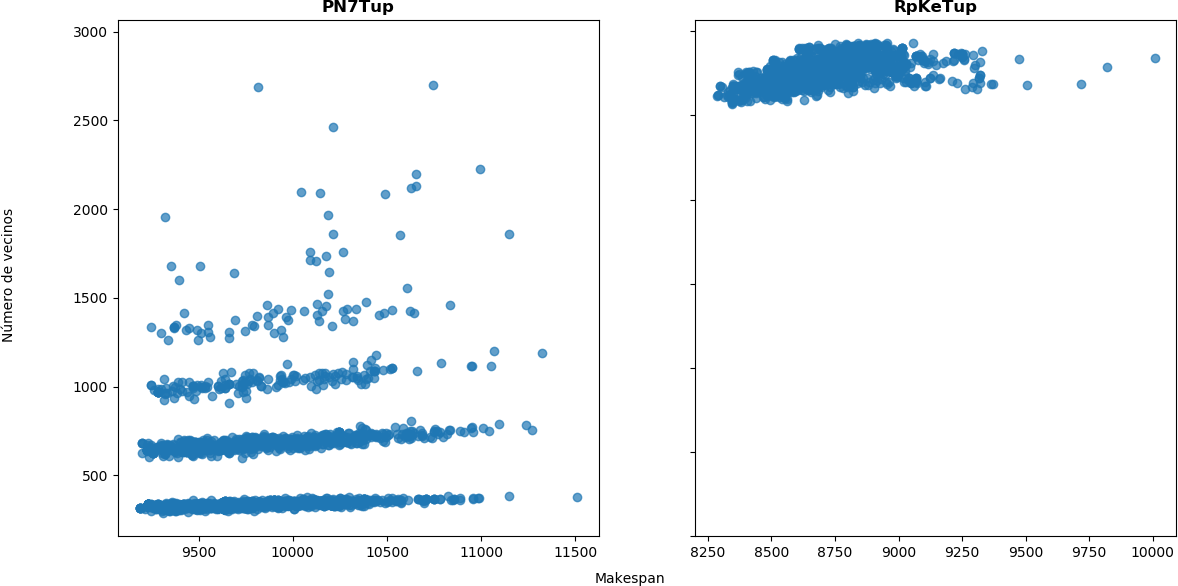
\includegraphics[scale=.6]{Imagenes/compvec78.png}
    \caption{Comparación de tamaño de la vecindad contra makespan de los óptimos locales para la instancia \textbf{DMU78} }
    \label{fig:mattgraph}
\end{figure}

Otro modo de visualizar las diferencias entre ambas representaciones es al fijarnos en los alrededores de un óptimo local. Entre más parecido se el makespan de un óptimo local al de sus vecinos, más suave es el paisaje de búsqueda. Podemos visualizar esto mediante diagramas de caja para la diferencia relativa relativa del makespan de los óptimos locales con sus vecinos. 

En las figuras \ref{fig:bxp1} y \ref{fig:bxp2} observamos que los vecinos de los óptimos locales para \textbf{RpKeTup} son más parecidos que los de \textbf{PN7Tup}, esto nos indica que el paisaje de búsqueda es más suave para \textbf{RpKeTup} lo cual, como se ha mencionado antes, es ventajoso para las metaheurísticas de trayectoria.  

Este efecto se debe a que la representación basada en permutaciones considera movimientos que pueden ser bastante disruptivos como atrasar toda una cadena de operaciones dejando huecos grandes en la planificación, mientras que en la nueva representación basada en llaves aleatorias el proceso de decodificación mediante el algoritmo de Giffler Thompson \ref{alg:GT} evita que se generen estos huecos lo que tiene como resultado un paisaje de búsqueda mucho más suave.
\begin{figure}[hbtp]
    \begin{subfigure}{\textwidth}
        \centering
        %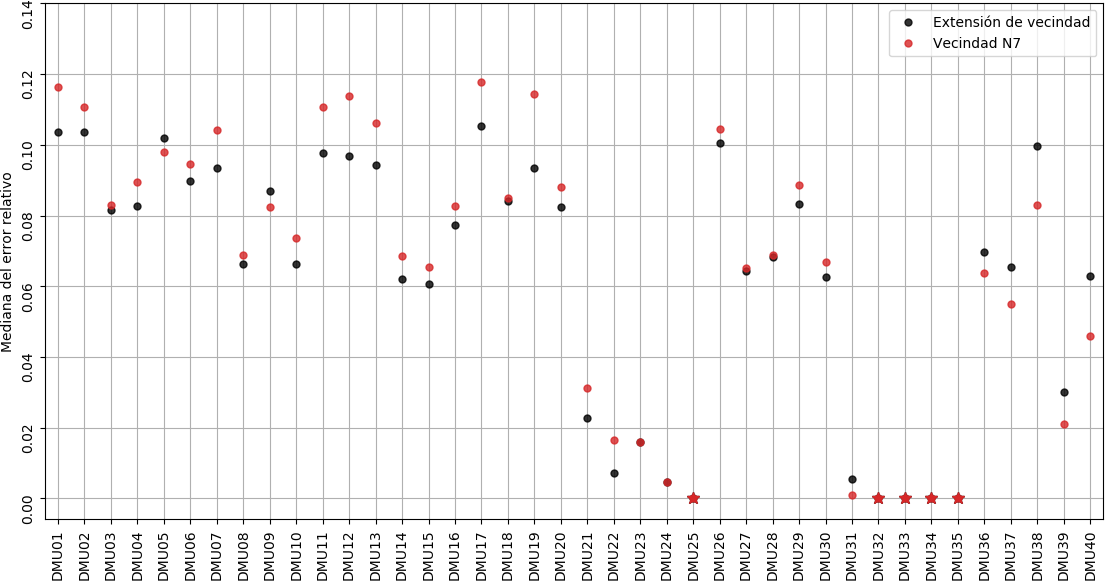
\includegraphics[height=.78\textwidth,width=.95\textheight,angle=270]{Imagenes/n8vsn7err1.png}
        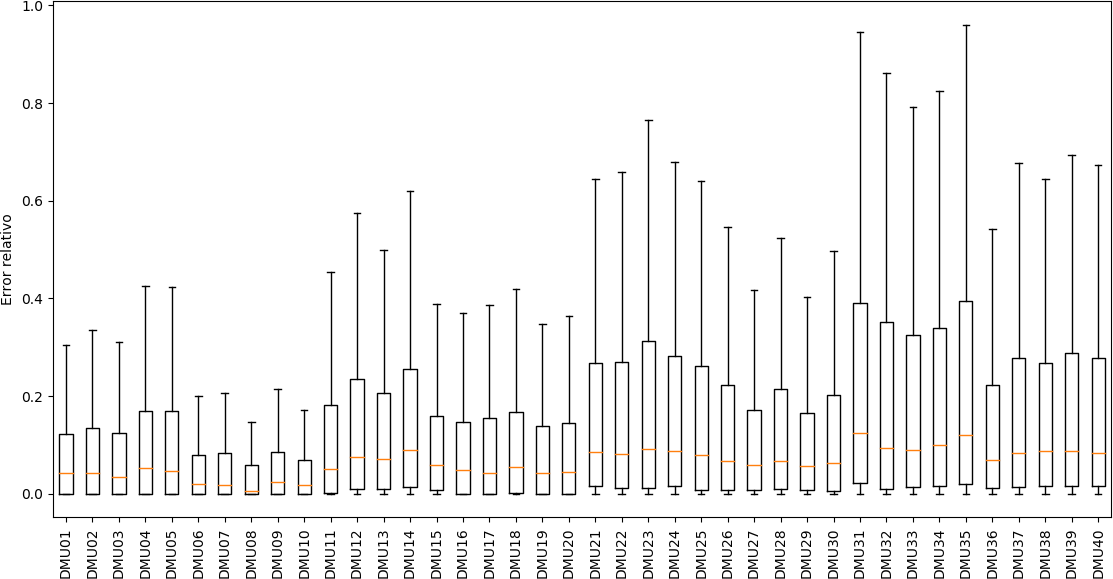
\includegraphics[scale=.6]{Imagenes/bxpn7_1.png}
        \caption{Representación original con vecindad n7 instancias \textbf{DMU01-40}}
    \end{subfigure}
\end{figure}
\begin{figure}[H]\ContinuedFloat
    \begin{subfigure}{\textwidth}
        \centering
        %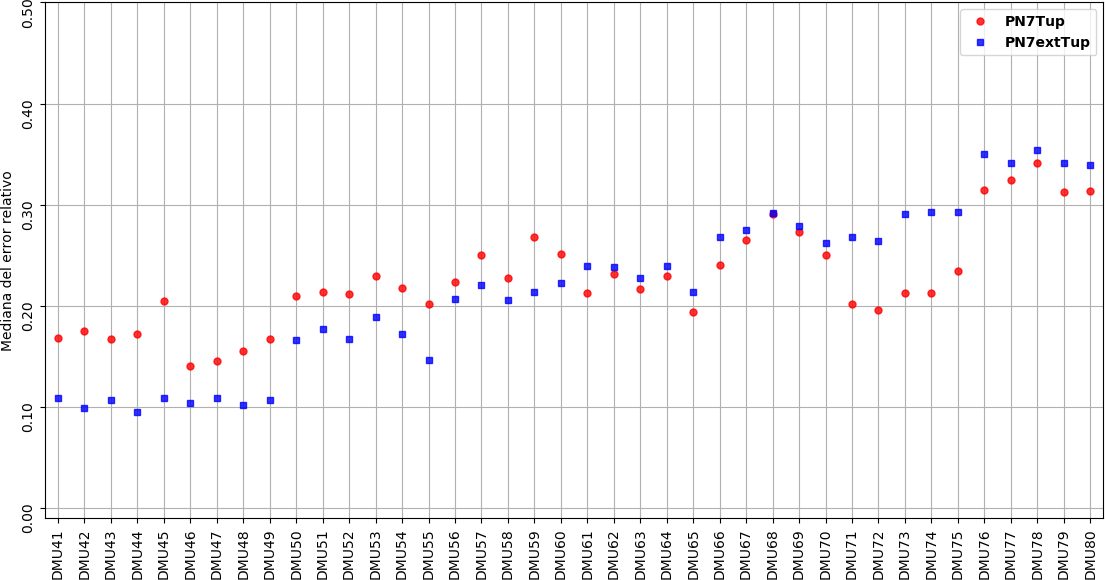
\includegraphics[height=.78\textwidth,width=.95\textheight,angle=270]{Imagenes/n8vsn7err2.png}
        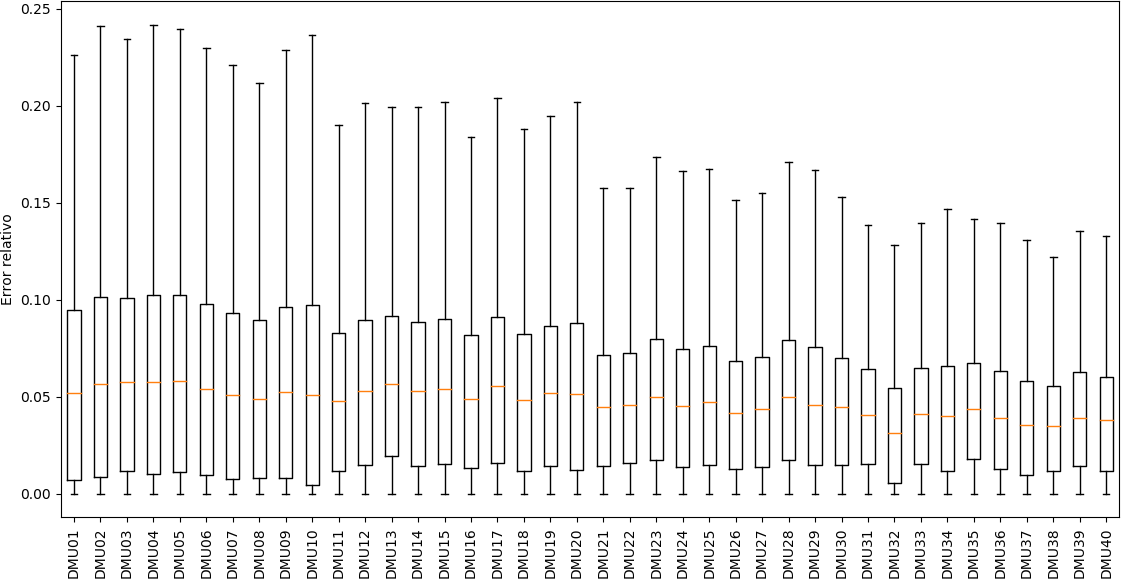
\includegraphics[scale=.6]{Imagenes/bxppr_1.png}
        \caption{Representación propuesta instancias \textbf{DMU01-40}}
    \end{subfigure}
    \caption{Diagramas de caja de la diferencia relativa en makespan de un óptimo local con sus vecinos}
    \label{fig:bxp1}
\end{figure}


\begin{figure}[hbtp]
    \begin{subfigure}{\textwidth}
        \centering
        %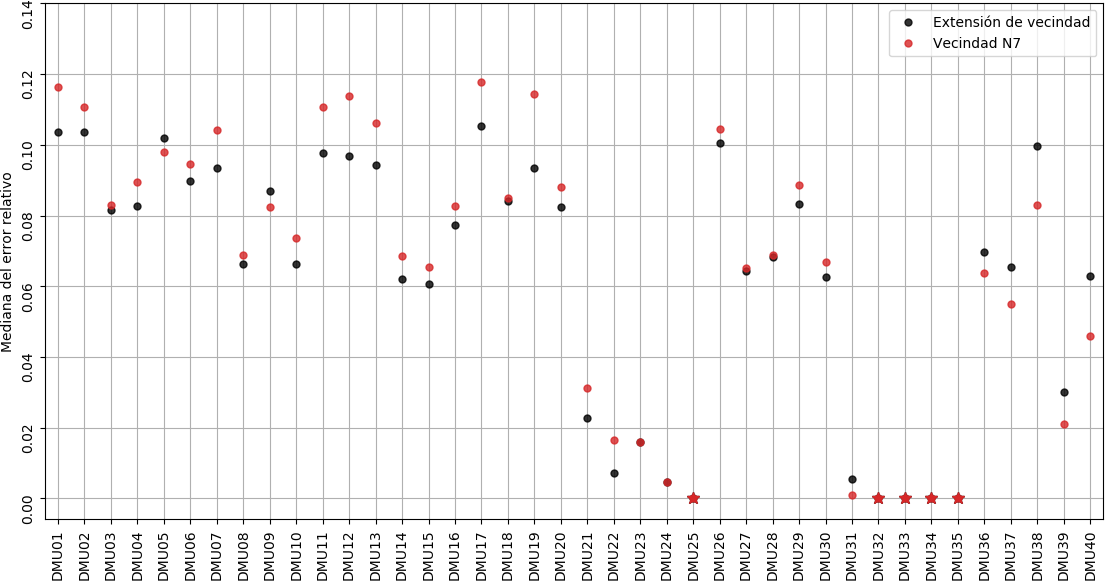
\includegraphics[height=.78\textwidth,width=.95\textheight,angle=270]{Imagenes/n8vsn7err1.png}
        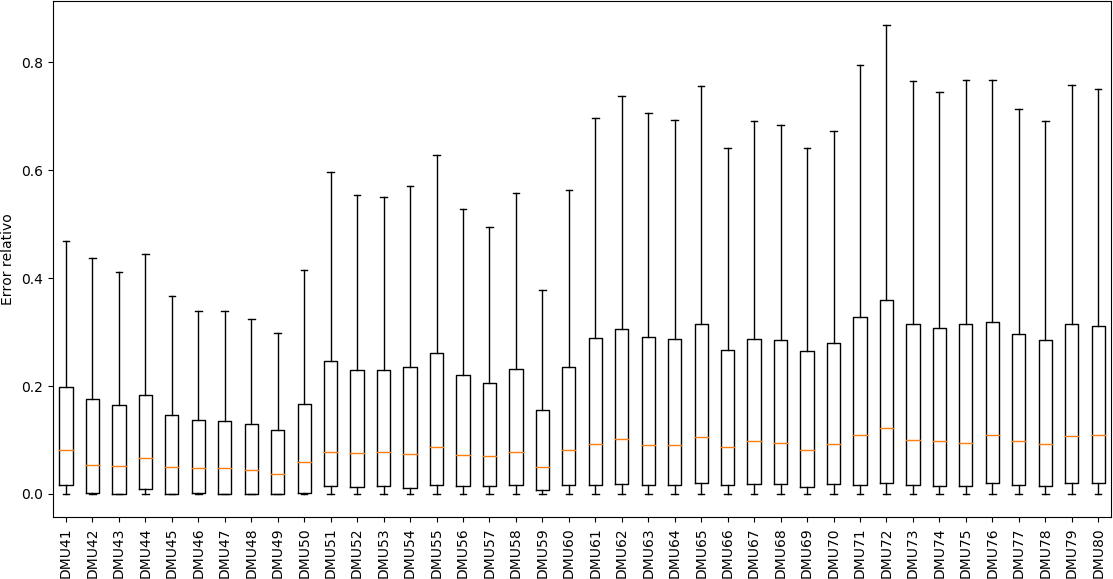
\includegraphics[scale=.6]{Imagenes/bxpn7_2.png}
        \caption{Representación original con vecindad n7 instancias \textbf{DMU41-80}}
    \end{subfigure}
\end{figure}
\begin{figure}[H]\ContinuedFloat
    \begin{subfigure}{\textwidth}
        \centering
        %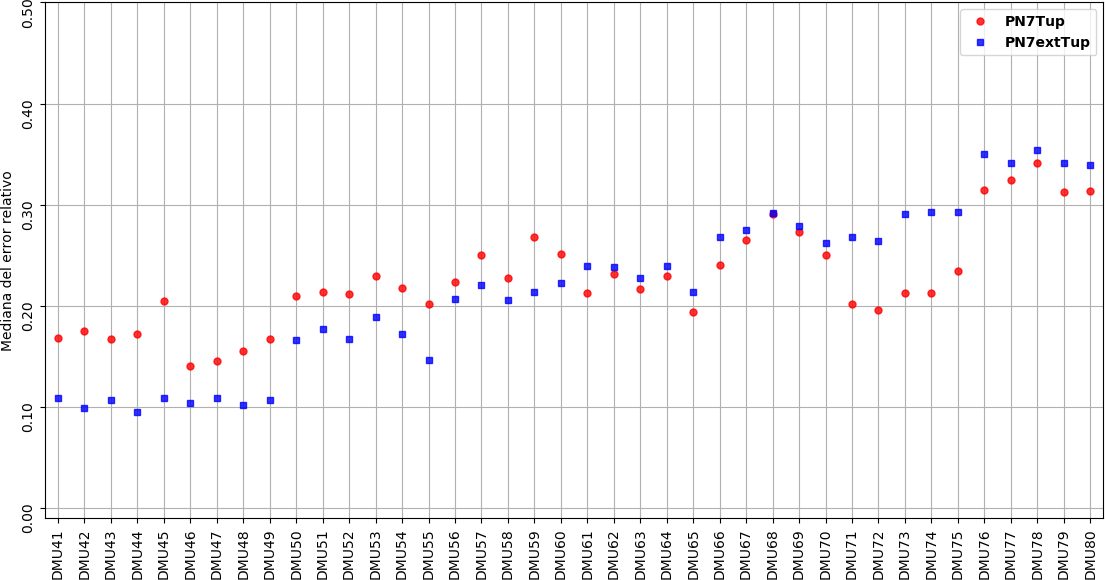
\includegraphics[height=.78\textwidth,width=.95\textheight,angle=270]{Imagenes/n8vsn7err2.png}
        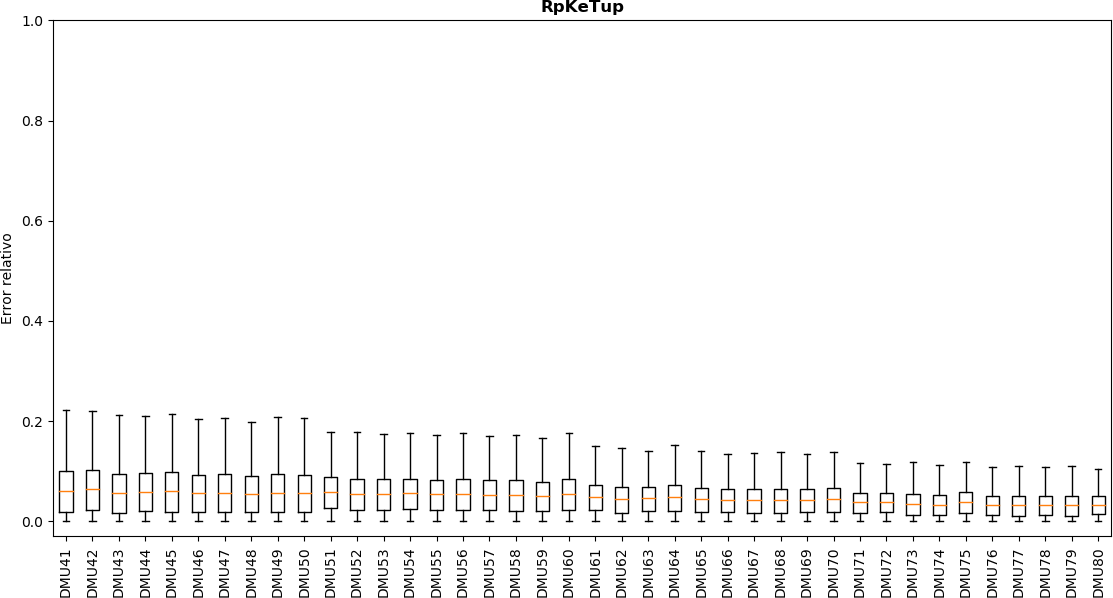
\includegraphics[scale=.6]{Imagenes/bxppr_2.png}
        \caption{Representación propuesta instancias \textbf{DMU41-80}}
    \end{subfigure}
    \caption{Diagramas de caja de la diferencia relativa en makespan de un óptimo local con sus vecinos}
    \label{fig:bxp2}
\end{figure}

